\section{Einpuls-Gleichrichter}

\subsection{M1U: Ungesteuerter Einpuls-Gleichrichter}

% --- bestehende Grafik: Schaltung ---
Einpuls-Gleichrichter M1U
\begin{center}
    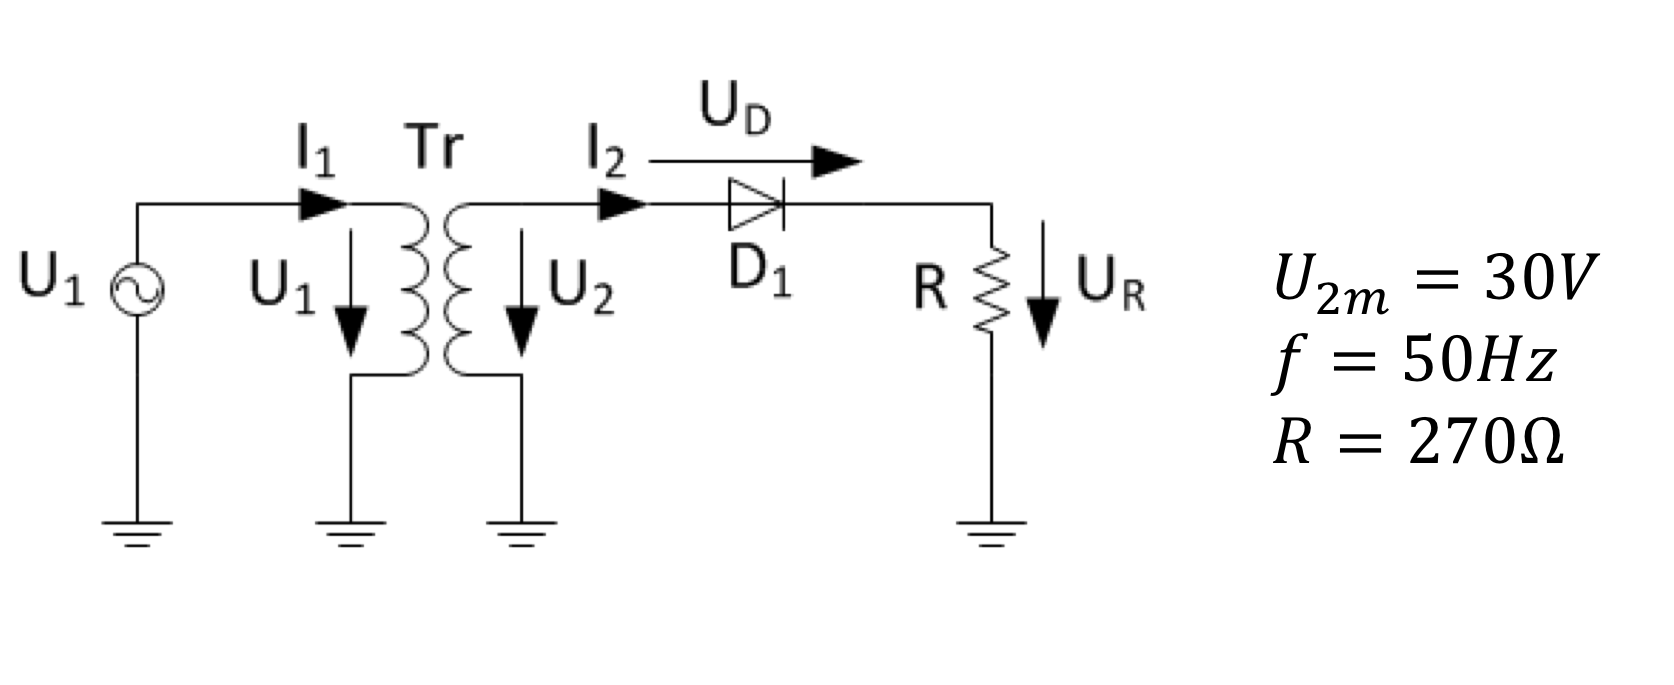
\includegraphics[width=0.85\linewidth]{images/M1U.png}
\end{center}

Der ungesteuerte Einpuls-Gleichrichter besteht aus einer Diode und einer Wechselspannungsquelle.
Er liefert eine pulsierende Gleichspannung mit einer Pulszahl von $p=1$.

Momentane Ausgangsspannung:
\[
u_d(t) =
\begin{cases}
u_s(t), & u_s(t) \ge 0 \\
0, & u_s(t) < 0
\end{cases}
\]

Mittelwert:
\[
\cbl{\overline{u_d} = \frac{\hat U}{\pi}}
\]

Effektivwert:
\[
\cbl{U_{d,\mathrm{RMS}} = \frac{\hat U}{2}}
\]

Eigenschaften:
\begin{itemize}
    \item Keine Stellmöglichkeit
    \item Starke Welligkeit der Gleichspannung
    \item Einfachste Gleichrichterschaltung
\end{itemize}

% --- bestehende Grafik: Spannungsverlauf ---
\begin{center}

    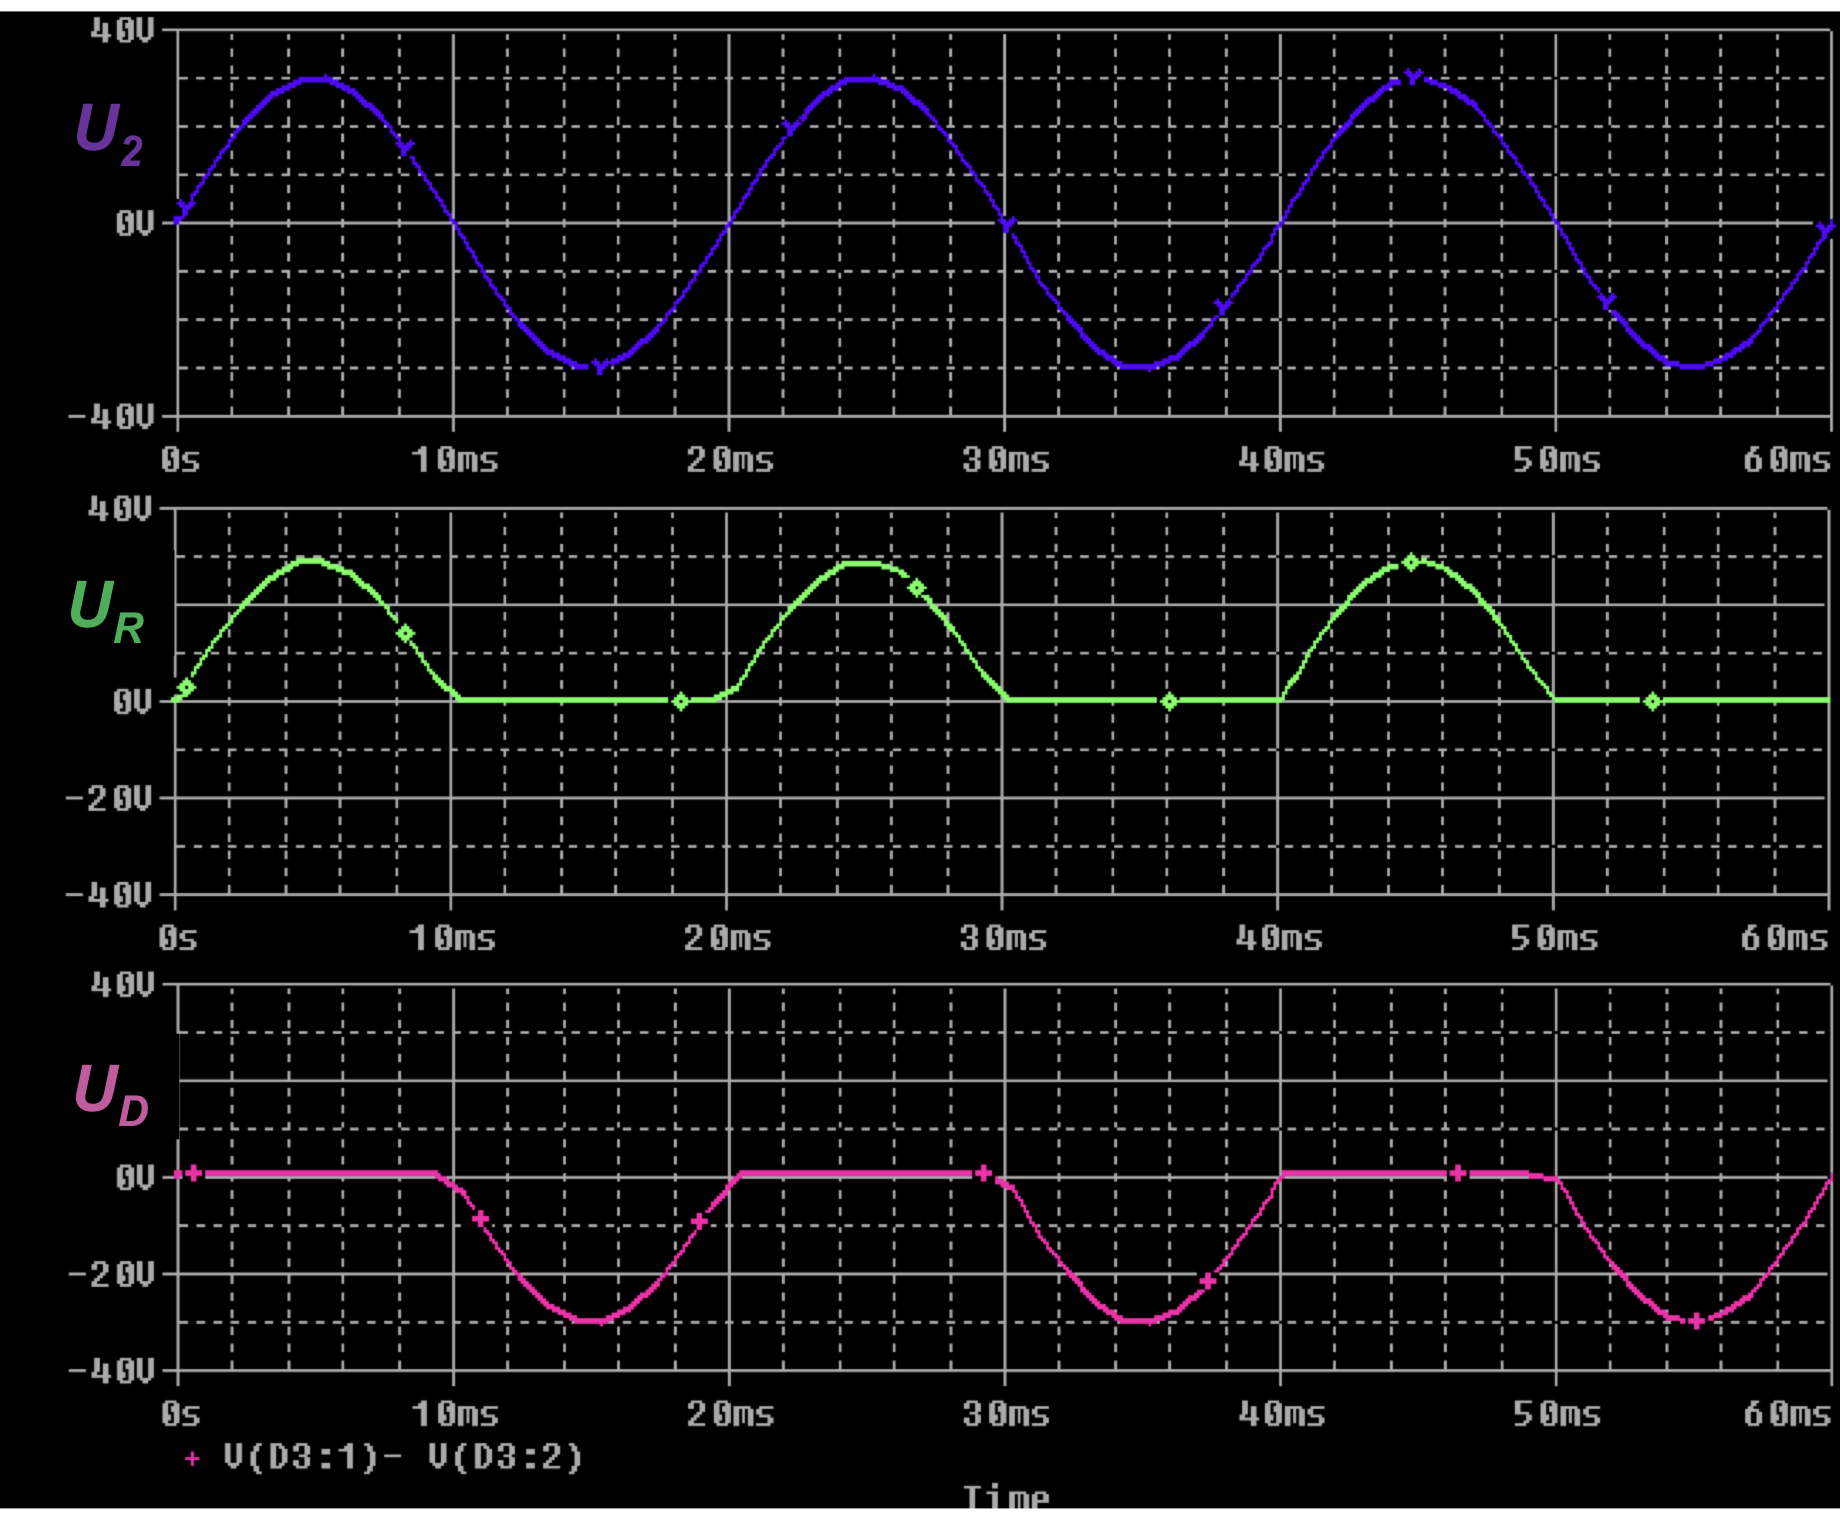
\includegraphics[width=0.85\linewidth]{images/M1U_verlauf.png}

\end{center}
Ausgangsspannung $u_d(t)$ beim M1U
% -------------------------------------------------
\subsection{M1U mit kapazitiver Last}

Bei kapazitiver Last leitet die Diode nur während eines kurzen Intervalls um das Spannungsmaximum.
Zwischen zwei Leitphasen entlädt sich der Kondensator über den Widerstand.

\paragraph{Sperrphase der Diode}

Für die Sperrphase gilt die Differentialgleichung:

\[
\frac{u_R(t)}{R} + C \frac{du_R(t)}{dt} = 0
\]

mit der Zeitkonstante:

\[
\cbl{\tau = RC}
\]

Lösung der Differentialgleichung:

\[
\cbl{u_R(t) = B \, e^{-t/\tau}}
\]

\paragraph{Ausschaltwinkel}

Der Ausschaltwinkel $\beta_a$ ergibt sich aus:

\[
\cbl{\tan \beta_a = - \omega \tau}
\]

\paragraph{Einschaltwinkel}

Der Einschaltwinkel $\beta_e$ folgt aus der Bedingung:

\[
\cbl{U_{2m} \sin \beta_e = U_{2m} \sin \beta_a \, e^{(\beta_a - \beta_e)/(\omega \tau)}}
\]

Dies ist eine transzendente Gleichung und wird numerisch oder grafisch gelöst.

\crd{\textrightarrow\ Diese Methode wird direkt in Prüfungen für M1U mit C-Last verwendet.}

\subsection{M1C: Gesteuerter Einpuls-Gleichrichter}

% --- bestehende oder neue Grafik: Thyristor-Schaltung ---
Gesteuerter Einpuls-Gleichrichter M1C
\begin{center}
    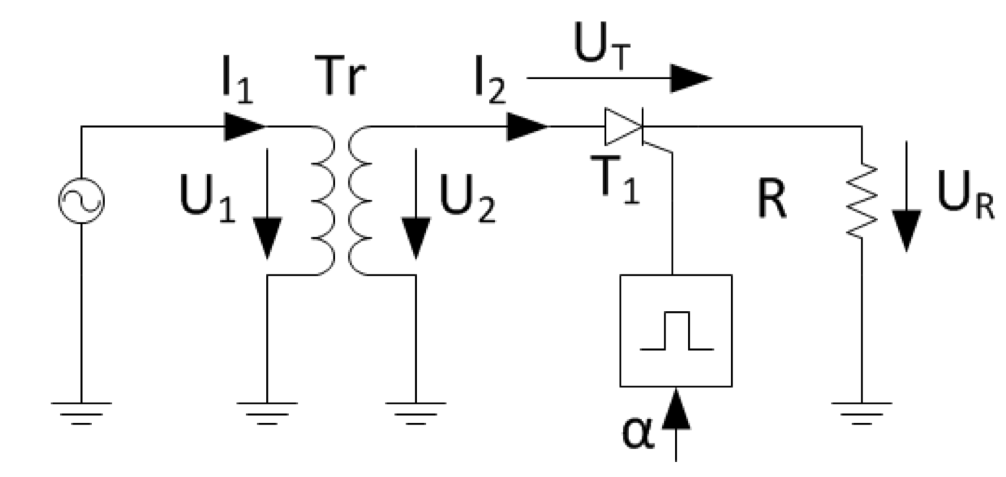
\includegraphics[width=0.85\linewidth]{images/M1C.png}
\end{center}

Beim gesteuerten Einpuls-Gleichrichter wird die Diode durch einen Thyristor ersetzt.
Die Gleichspannung ist über den Zündwinkel $\alpha$ steuerbar.

Momentane Ausgangsspannung:
\[
u_d(t) =
\begin{cases}
u_s(t), & \omega t \ge \alpha \\
0, & \omega t < \alpha
\end{cases}
\]

Mittelwert:
\[
\cbl{\overline{u_d} = \frac{\hat U}{2\pi}(1+\cos\alpha)}
\]

Eigenschaften:
\begin{itemize}
    \item Stellbereich: $0 \le \alpha \le \pi$
    \item Bei $\alpha = 0$: maximaler Mittelwert
    \item Bei $\alpha = \pi$: $\overline{u_d} = 0$
\end{itemize}

\crd{\textrightarrow\ M1C ist der einfachste gesteuerte Gleichrichter.}
